% answers.tex —— 2007 年·普通高等学校招生考试·浙江卷·理科 · 参考答案与详细解析片段
% 由 tools/generate_projects.py 依来源总账自 2007/2007_数学真题_浙江理_试题.md + 2007/2007_数学真题_浙江理_解析正文.md + 2007/2007_数学真题_浙江理_答案要点.md 生成，勿手改（改源 MD 后重跑）


\begin{gktip}
固定候选 PDF 仅含题面，无答案、解析和评分标准，原卷亦未标注分值；以下为非官方编者独立推导，官方答案字段为空。来源发布者、出版者、版次与官方身份均未核。
\end{gktip}

\begin{answer}
\gksolhead{1}{}

\textbf{题目}：

“$x>1$”是“$x^2>x$”的（　）

（A）充分而不必要条件

（B）必要而不充分条件

（C）充分必要条件

（D）既不充分也不必要条件

\Needspace{4\baselineskip}
\textbf{解析}

$x>1\Rightarrow x(x-1)>0\Rightarrow x^2>x$；反之 $x^2>x$ 还得 $x<0$。故为充分而不必要条件。

\gkanswer{答案：A。}

\end{answer}
\begin{answer}
\gksolhead{2}{}

\textbf{题目}：

若函数 $f(x)=2\sin(\omega x+\varphi)$，$x\in\mathbf R$（其中 $\omega>0$，$|\varphi|<\dfrac{\pi}{2}$）的最小正周期是 $\pi$，且 $f(0)=\sqrt3$，则（　）

（A）$\omega=\dfrac12$，$\varphi=\dfrac{\pi}{6}$

（B）$\omega=\dfrac12$，$\varphi=\dfrac{\pi}{3}$

（C）$\omega=2$，$\varphi=\dfrac{\pi}{6}$

（D）$\omega=2$，$\varphi=\dfrac{\pi}{3}$

\Needspace{4\baselineskip}
\textbf{解析}

周期 $\pi=\dfrac{2\pi}{\omega}$，故 $\omega=2$。又 $f(0)=2\sin\varphi=\sqrt3$，$\sin\varphi=\dfrac{\sqrt3}{2}$，结合 $|\varphi|<\dfrac{\pi}{2}$ 得 $\varphi=\dfrac{\pi}{3}$。

\gkanswer{答案：D。}

\end{answer}
\begin{answer}
\gksolhead{3}{}

\textbf{题目}：

直线 $x-2y+1=0$ 关于直线 $x=1$ 对称的直线方程是（　）

（A）$x+2y-1=0$

（B）$2x+y-1=0$

（C）$2x+y-3=0$

（D）$x+2y-3=0$

\Needspace{4\baselineskip}
\textbf{解析}

把 $x$ 换成 $2-x$：$(2-x)-2y+1=0$，即 $x+2y-3=0$。

\gkanswer{答案：D。}

\end{answer}
\begin{answer}
\gksolhead{4}{}

\textbf{题目}：

要在边长为 $16$ 米的正方形草坪上安装喷水龙头，使整个草坪都能喷洒到水。假设每个喷水龙头的喷洒范围都是半径为 $6$ 米的圆面，则需安装这种喷水龙头的个数最少是（　）
\nopagebreak[4]
\begin{center}% 2007 年浙江卷理科第 4 题：边长 16 米的正方形草坪与喷水龙头示意。
% 来源 PDF：gaokaomath-src/普通高考/2007/2007浙江理.pdf
% SHA-256：31c1d0d79ba11a3644a27b5ee3781f52caaf831209e8da63ddd8d7019cd06995
% 原页：2007浙江理.pdf 第 1 页（A3 三栏）第 1 栏，书页码 417。
% 重绘依据：按原页正方形草坪与中心喷水圆面的透视重绘。
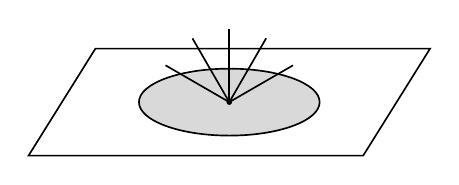
\begin{tikzpicture}[scale=0.85, semithick,
  every node/.style={inner sep=1pt}]

  % 正方形草坪（斜投影）
  \draw (0,0) -- (5,0) -- (6,1.6) -- (1,1.6) -- cycle;

  % 喷水圆面
  \fill[gray!30] (3,0.8) ellipse (1.35 and 0.5);
  \draw (3,0.8) ellipse (1.35 and 0.5);
  \fill (3,0.8) circle (1.2pt);

  % 水花射线
  \foreach \a in {30,60,90,120,150} {
    \draw (3,0.8) -- ++(\a:1.1);
  }
\end{tikzpicture}
\end{center}
\nopagebreak[4]
（A）$3$

（B）$4$

（C）$5$

（D）$6$

\Needspace{4\baselineskip}
\textbf{解析}

一个半径 $6$ 的圆不能同时覆盖相距 $16$ 的两个顶点，四个顶点需四个圆；四圆圆心取四个 $8\times8$ 小正方形中心时，顶点到圆心 $4\sqrt2<6$，可覆盖。最少 $4$ 个。

\gkanswer{答案：B。}

\end{answer}
\begin{answer}
\gksolhead{5}{}

\textbf{题目}：

已知随机变量 $\xi$ 服从正态分布 $N(2,\sigma^2)$，$P(\xi\leqslant4)=0.84$，则 $P(\xi\leqslant0)=$（　）

（A）$0.16$

（B）$0.32$

（C）$0.68$

（D）$0.84$

\Needspace{4\baselineskip}
\textbf{解析}

正态曲线关于 $\xi=2$ 对称，$P(\xi\leqslant0)=P(\xi\geqslant4)=1-P(\xi\leqslant4)=0.16$。

\gkanswer{答案：A。}

\end{answer}
\begin{answer}
\gksolhead{6}{}

\textbf{题目}：

若 $P$ 是两条异面直线 $l$，$m$ 外的任意一点，则（　）

（A）过点 $P$ 有且仅有一条直线与 $l$，$m$ 都平行

（B）过点 $P$ 有且仅有一条直线与 $l$，$m$ 都垂直

（C）过点 $P$ 有且仅有一条直线与 $l$，$m$ 都相交

（D）过点 $P$ 有且仅有一条直线与 $l$，$m$ 都异面

\Needspace{4\baselineskip}
\textbf{解析}

异面直线方向向量不平行，过 $P$ 与两方向都垂直的方向唯一（叉乘方向），故有且仅有一条。

\gkanswer{答案：B。}

\end{answer}
\begin{answer}
\gksolhead{7}{}

\textbf{题目}：

若非零向量 $\boldsymbol a$，$\boldsymbol b$ 满足 $|\boldsymbol a+\boldsymbol b|=|\boldsymbol b|$，则（　）

（A）$|2\boldsymbol a|>|2\boldsymbol a+\boldsymbol b|$

（B）$|2\boldsymbol a|<|2\boldsymbol a+\boldsymbol b|$

（C）$|2\boldsymbol b|>|\boldsymbol a+2\boldsymbol b|$

（D）$|2\boldsymbol b|<|\boldsymbol a+2\boldsymbol b|$

\Needspace{4\baselineskip}
\textbf{解析}

\Needspace{5\baselineskip}
由 $|\boldsymbol a+\boldsymbol b|=|\boldsymbol b|$ 得

\nopagebreak[4]
\[\boldsymbol a^2+2\boldsymbol a\cdot\boldsymbol b=0\ \Rightarrow\ \boldsymbol a\cdot\boldsymbol b=-\frac{\boldsymbol a^2}{2}.\]

\Needspace{5\baselineskip}
于是

\nopagebreak[4]
\[|\boldsymbol a+2\boldsymbol b|^2=\boldsymbol a^2+4\boldsymbol a\cdot\boldsymbol b+4\boldsymbol b^2=4\boldsymbol b^2-\boldsymbol a^2<4\boldsymbol b^2,\]

故 $|2\boldsymbol b|>|\boldsymbol a+2\boldsymbol b|$。

\gkanswer{答案：C。}

\end{answer}
\begin{answer}
\gksolhead{8}{}

\textbf{题目}：

设 $f'(x)$ 是函数 $f(x)$ 的导函数，将 $y=f(x)$ 和 $y=f'(x)$ 的图象画在同一个直角坐标系中，不可能正确的是（　）
\nopagebreak[4]
\begin{center}% 2007 年浙江卷理科第 8 题：y=f(x) 与 y=f'(x) 在同一坐标系中的四个图象选项。
%   （A）f=x^2 与 f'=2x；（B）f 单调递减而 f' 取正值（不可能）；
%   （C）f=e^x 与 f'=e^x；（D）f 为四次型曲线、f' 在其极值点变号。
% 来源 PDF：gaokaomath-src/普通高考/2007/2007浙江理.pdf
% SHA-256：3b1e5fbca7888b1cff1fc809211aac94f14ea503de0229c4edf7cfb54e5bd2d4
% 原页：2007浙江理.pdf 第 1 页（A3 三栏）第 2 栏，书页码 417。
% 重绘依据：按原页四个小图的曲线形状、相对位置与坐标轴重绘。
\begin{tikzpicture}[scale=0.9, semithick,
  every node/.style={inner sep=1pt, font=\small}]

  % ---------------- （A） ----------------
  \begin{scope}[shift={(0,0)}]
    \draw[->,>=stealth] (-1.8,0) -- (2.1,0) node[right] {$x$};
    \draw[->,>=stealth] (0,-1.4) -- (0,1.8) node[above] {$y$};
    \draw[domain=-1.25:1.25,samples=100] plot (\x,{\x*\x});
    \draw (-1.5,-1.2) -- (1.5,1.2);
    \node[below] at (0.8,-1.7) {（A）};
  \end{scope}

  % ---------------- （B） ----------------
  \begin{scope}[shift={(4.6,0)}]
    \draw[->,>=stealth] (-1.8,0) -- (2.1,0) node[right] {$x$};
    \draw[->,>=stealth] (0,-1.4) -- (0,1.8) node[above] {$y$};
    \draw[domain=-1.4:1.4,samples=100] plot (\x,{1.3*exp(-0.7*(\x+0.2))});
    \draw[domain=-1.4:1.4,samples=100] plot (\x,{0.9*(\x-0.1)});
    \node[below] at (0.8,-1.7) {（B）};
  \end{scope}

  % ---------------- （C） ----------------
  \begin{scope}[shift={(0,-4.4)}]
    \draw[->,>=stealth] (-1.8,0) -- (2.1,0) node[right] {$x$};
    \draw[->,>=stealth] (0,-1.4) -- (0,1.8) node[above] {$y$};
    \draw[domain=-1.3:0.55,samples=100] plot (\x,{0.55*exp(1.1*\x)});
    \draw[domain=-0.2:1.2,samples=100] plot (\x,{0.65*exp(0.8*\x)});
    \node[below] at (0.8,-1.7) {（C）};
  \end{scope}

  % ---------------- （D） ----------------
  \begin{scope}[shift={(4.6,-4.4)}]
    \draw[->,>=stealth] (-1.8,0) -- (2.1,0) node[right] {$x$};
    \draw[->,>=stealth] (0,-1.4) -- (0,1.8) node[above] {$y$};
    \draw[domain=-1.4:1.5,samples=120]
      plot (\x,{0.9*cos(deg(2.2*\x))});
    \draw[domain=-1.4:1.5,samples=120]
      plot (\x,{0.55*sin(deg(2.2*\x))});
    \node[below] at (0.8,-1.7) {（D）};
  \end{scope}
\end{tikzpicture}
\end{center}
\nopagebreak[4]
\Needspace{4\baselineskip}
\textbf{解析}

若 $f(x)$ 在区间上单调递减，则 $f'(x)\leqslant0$，其图象应在 $x$ 轴下方或与 $x$ 轴接触。选项（B）中一条曲线单调递减（$f$），另一条曲线在部分区间取正值（$f'$），这与“$f$ 递减时 $f'\leqslant0$”矛盾，故不可能正确。

\gkanswer{答案：B。}

\end{answer}
\begin{answer}
\gksolhead{9}{}

\textbf{题目}：

已知双曲线 $\dfrac{x^2}{a^2}-\dfrac{y^2}{b^2}=1$（$a>0$，$b>0$）的左、右焦点分别为 $F_1$，$F_2$，$P$ 是准线上一点，且 $PF_1\perp PF_2$，$|PF_1|\cdot|PF_2|=4ab$，则双曲线的离心率是（　）

（A）$\sqrt2$

（B）$\sqrt3$

（C）$2$

（D）$3$

\Needspace{4\baselineskip}
\textbf{解析}

\Needspace{5\baselineskip}
设 $P$ 在右准线 $x=\dfrac{a^2}{c}$ 上。由 $PF_1\perp PF_2$ 得 $x_P^2+y_P^2=c^2$，故

\nopagebreak[4]
\[y_P^2=c^2-\frac{a^4}{c^2}.\]

\Needspace{5\baselineskip}
计算得

\nopagebreak[4]
\[|PF_1|^2=2(a^2+c^2),\qquad |PF_2|^2=2(c^2-a^2).\]

\Needspace{5\baselineskip}
由乘积条件：

\nopagebreak[4]
\[2\sqrt{c^4-a^4}=4ab\ \Rightarrow\ c^4-a^4=4a^2(c^2-a^2).\]

\Needspace{5\baselineskip}
令 $e=\dfrac ca$，得

\nopagebreak[4]
\[(e^2-1)(e^2-3)=0,\]

故 $e=\sqrt3$。

\gkanswer{答案：B。}

\end{answer}
\begin{answer}
\gksolhead{10}{}

\textbf{题目}：

设 $f(x)=\begin{cases}x^2,&|x|\geqslant1,\\ x,&|x|<1,\end{cases}$ 若 $f(g(x))$ 的值域是 $[0,+\infty)$，则函数 $g(x)$ 的值域是（　）

（A）$(-\infty,-1]\cup[1,+\infty)$

（B）$(-\infty,-1]\cup[0,+\infty)$

（C）$[0,+\infty)$

（D）$[1,+\infty)$

\Needspace{4\baselineskip}
\textbf{解析}

$f$ 的值域为 $(-1,+\infty)$。要使 $f(g(x))\in[0,+\infty)$，需 $g(x)\in[0,+\infty)$（若 $g(x)\in(-1,0)$，则 $f(g(x))=g(x)<0$）。又 $f$ 在 $[0,+\infty)$ 上取遍 $[0,+\infty)$，故 $g$ 的值域为 $[0,+\infty)$。

\gkanswer{答案：C。}

\end{answer}
\begin{answer}
\gksolhead{11}{}

\textbf{题目}：

已知复数 $z_1=1-\mathrm i$，$z_1\cdot z_2=1+\mathrm i$，则复数 $z_2=$\gkblank{}。

\Needspace{4\baselineskip}
\textbf{解析}

\nopagebreak[4]
\[z_2=\frac{1+\mathrm i}{1-\mathrm i}=\frac{(1+\mathrm i)^2}{2}=\mathrm i.\]

\gkanswer{答案：$\mathrm i$。}

\end{answer}
\begin{answer}
\gksolhead{12}{}

\textbf{题目}：

已知 $\sin\theta+\cos\theta=\dfrac15$，且 $\dfrac{\pi}{2}\leqslant\theta\leqslant\dfrac{3\pi}{4}$，则 $\cos2\theta$ 的值是\gkblank{}。

\Needspace{4\baselineskip}
\textbf{解析}

\Needspace{5\baselineskip}
平方得

\nopagebreak[4]
\[1+\sin2\theta=\frac1{25}\ \Rightarrow\ \sin2\theta=-\frac{24}{25}.\]

\Needspace{5\baselineskip}
由 $\theta\in\left[\dfrac{\pi}{2},\dfrac{3\pi}{4}\right]$ 得 $2\theta\in[\pi,3\pi/2]$，故 $\cos2\theta<0$：

\nopagebreak[4]
\[\cos2\theta=-\sqrt{1-\frac{576}{625}}=-\frac7{25}.\]

\gkanswer{答案：$-\dfrac7{25}$。}

\end{answer}
\begin{answer}
\gksolhead{13}{}

\textbf{题目}：

不等式 $|2x-1|-x<1$ 的解集是\gkblank{}。

\Needspace{4\baselineskip}
\textbf{解析}

\nopagebreak[4]
\[|2x-1|<x+1.\]

\Needspace{5\baselineskip}
先需 $x>-1$。再解

\nopagebreak[4]
\[-(x+1)<2x-1<x+1.\]

左半：$3x>0\Rightarrow x>0$；右半：$x<2$。故 $0<x<2$。

\gkanswer{答案：$(0,2)$。}

\end{answer}
\begin{answer}
\gksolhead{14}{}

\textbf{题目}：

某书店有 $11$ 种杂志，$2$ 元 $1$ 本的 $8$ 种，$1$ 元 $1$ 本的 $3$ 种。小张用 $10$ 元钱买杂志（每种至多买一本，$10$ 元钱刚好用完），则不同买法的种数是\gkblank{}。（用数字作答）

\Needspace{4\baselineskip}
\textbf{解析}

\Needspace{5\baselineskip}
设买 $2$ 元杂志 $k$ 本、$1$ 元 $m$ 本：

\nopagebreak[4]
\[2k+m=10,\qquad 0\leqslant k\leqslant8,\ 0\leqslant m\leqslant3.\]

\Needspace{5\baselineskip}
得 $(k,m)=(4,2),(5,0)$，故

\nopagebreak[4]
\[\mathrm C_8^4\mathrm C_3^2+\mathrm C_8^5=70\times3+56=266.\]

\gkanswer{答案：$266$。}

\end{answer}
\begin{answer}
\gksolhead{15}{}

\textbf{题目}：

随机变量 $\xi$ 的分布列如下：

\begin{center}
\begin{tabular}{llll}
\toprule
$\xi$ & $-1$ & $0$ & $1$ \\
\midrule
$P$ & $a$ & $b$ & $c$ \\
\bottomrule
\end{tabular}
\end{center}

其中 $a$，$b$，$c$ 成等差数列。若 $E\xi=\dfrac13$，则 $D\xi$ 的值是\gkblank{}。

\Needspace{4\baselineskip}
\textbf{解析}

\Needspace{5\baselineskip}
由分布列，

\nopagebreak[4]
\[a+b+c=1.\]

$a,b,c$ 成等差数列，故 $2b=a+c$，于是 $3b=1$，$b=\dfrac13$。

\Needspace{5\baselineskip}
又

\nopagebreak[4]
\[E\xi=-a+c=\frac13.\]

\Needspace{5\baselineskip}
结合 $a+c=\dfrac23$ 解得 $a=\dfrac16$，$c=\dfrac12$。于是

\nopagebreak[4]
\[E\xi^2=a+c=\frac23,\]

\nopagebreak[4]
\[D\xi=E\xi^2-(E\xi)^2=\frac23-\frac19=\frac59.\]

\gkanswer{答案：$\dfrac59$。}

\end{answer}
\begin{answer}
\gksolhead{16}{}

\textbf{题目}：

已知点 $O$ 在二面角 $\alpha-AB-\beta$ 的棱上，点 $P$ 在 $\alpha$ 内，且 $\angle POB=45^\circ$。若对于 $\beta$ 内异于 $O$ 的任意一点 $Q$，都有 $\angle POQ\geqslant45^\circ$，则二面角 $\alpha-AB-\beta$ 的大小是\gkblank{}。

\Needspace{4\baselineskip}
\textbf{解析}

\Needspace{5\baselineskip}
设二面角为 $\varphi$。$OP$ 与 $\beta$ 内离它最近的射线夹角为 $OP$ 与 $\beta$ 的夹角；题设要求该最小角为 $45^\circ$。取 $\beta$ 内垂直于棱的射线 $OB'$，则

\nopagebreak[4]
\[\angle POB'=45^\circ,\]

即二面角为 $45^\circ$。

\gkanswer{答案：$45^\circ$。}

\end{answer}
\begin{answer}
\gksolhead{17}{}

\textbf{题目}：

设 $m$ 为实数，若 $\left\{(x,y)\ \middle|\ \begin{cases}x-2y+5\geqslant0,\\ 3-x\geqslant0,\\ mx+y\geqslant0\end{cases}\right\}\subseteq\{(x,y)\mid x^2+y^2\leqslant25\}$，则 $m$ 的取值范围是\gkblank{}。

\Needspace{4\baselineskip}
\textbf{解析}

\Needspace{5\baselineskip}
可行域由三条直线围成：

\nopagebreak[4]
\[L_1:\ x-2y+5=0,\qquad L_2:\ x=3,\qquad L_3:\ mx+y=0.\]

\Needspace{5\baselineskip}
$L_1$ 与 $L_2$ 交于 $(3,4)$；$L_2$ 与 $L_3$ 交于 $(3,-3m)$；$L_1$ 与 $L_3$ 交于

\nopagebreak[4]
\[\left(-\frac5{1+2m},\frac{5m}{1+2m}\right).\]

\Needspace{5\baselineskip}
三个顶点都需在圆 $x^2+y^2\leqslant25$ 内。$(3,4)$ 恰在圆上；$(3,-3m)$ 给出

\nopagebreak[4]
\[9+9m^2\leqslant25\ \Rightarrow\ |m|\leqslant\frac43.\]

\Needspace{5\baselineskip}
第三个顶点给出

\nopagebreak[4]
\[\frac{25(1+m^2)}{(1+2m)^2}\leqslant25\ \Rightarrow\ m(1+m)\geqslant0.\]

\Needspace{5\baselineskip}
又可行域有界要求 $m\geqslant0$。综合得

\nopagebreak[4]
\[0\leqslant m\leqslant\frac43.\]

\gkanswer{答案：$\left[0,\dfrac43\right]$。}

\end{answer}
\begin{answer}
\gksolhead{18}{}

\textbf{题目}：

已知 $\triangle ABC$ 的周长为 $\sqrt2+1$，且 $\sin A+\sin B=\sqrt2\sin C$。

（1）求边 $AB$ 的长；

（2）若 $\triangle ABC$ 的面积为 $\dfrac16\sin C$，求角 $C$ 的度数。

\Needspace{4\baselineskip}
\textbf{解析}

\Needspace{5\baselineskip}
（1）由正弦定理 $a+b=\sqrt2c$，周长

\nopagebreak[4]
\[(\sqrt2+1)c=\sqrt2+1\ \Rightarrow\ c=AB=1.\]

\Needspace{5\baselineskip}
（2）面积

\nopagebreak[4]
\[\frac12ab\sin C=\frac16\sin C\ \Rightarrow\ ab=\frac13.\]

\Needspace{5\baselineskip}
由余弦定理

\nopagebreak[4]
\[1=(a+b)^2-2ab(1+\cos C)=2-\frac23(1+\cos C),\]

得 $\cos C=\dfrac12$，故 $C=60^\circ$。

\gkanswer{答案：（1）$AB=1$；（2）$C=60^\circ$。}

\end{answer}
\begin{answer}
\gksolhead{19}{}

\textbf{题目}：

在如图所示的几何体中，$EA\perp$ 平面 $ABC$，$DB\perp$ 平面 $ABC$，$AC\perp BC$，且 $AC=BC=BD=2AE$，$M$ 是 $AB$ 的中点。

（1）求证：$CM\perp EM$；

（2）求 $CM$ 与平面 $CDE$ 所成的角。
\nopagebreak[4]
\begin{center}% 2007 年浙江卷理科第 19 题：EA、DB 均垂直于平面 ABC，AC⊥BC，M 为 AB 中点。
%   按 AC=BC=2、AE=1、BD=2 的示意比例绘制。
% 来源 PDF：gaokaomath-src/普通高考/2007/2007浙江理.pdf
% SHA-256：31c1d0d79ba11a3644a27b5ee3781f52caaf831209e8da63ddd8d7019cd06995
% 原页：2007浙江理.pdf 第 2 页（A3 三栏）第 1 栏，书页码 418。
% 重绘依据：按原页 C、A、B 底面与 E、D 的竖直位置重绘。
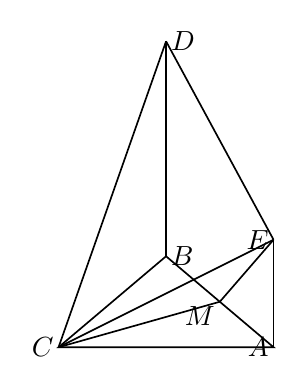
\begin{tikzpicture}[scale=1.05, semithick,
  every node/.style={inner sep=1.5pt}]

  \coordinate (C) at (0,0);
  \coordinate (A) at (2.6,0);
  \coordinate (B) at (1.3,1.1);
  \coordinate (E) at (2.6,1.3);
  \coordinate (D) at (1.3,3.7);
  \coordinate (M) at (1.95,0.55);

  % 底面
  \draw (C) -- (A) -- (B) -- cycle;
  % 竖直线
  \draw (A) -- (E);
  \draw (B) -- (D);
  % 上方连线
  \draw (E) -- (D);
  \draw (E) -- (C);
  \draw (D) -- (C);
  % 中点 M 相关
  \draw (C) -- (M);
  \draw (E) -- (M);

  \node[left] at (C) {$C$};
  \node[left] at (A) {$A$};
  \node[right] at (B) {$B$};
  \node[left] at (E) {$E$};
  \node[right] at (D) {$D$};
  \node[below left] at (M) {$M$};
\end{tikzpicture}
\end{center}
\nopagebreak[4]
\Needspace{4\baselineskip}
\textbf{解析}

\Needspace{5\baselineskip}
设 $AC=BC=2$，则 $AE=1$，$BD=2$。以 $C$ 为原点，$CA$，$CB$ 为 $x$，$y$ 轴，竖直向上为 $z$ 轴：

\nopagebreak[4]
\[C(0,0,0),\ A(2,0,0),\ B(0,2,0),\ E(2,0,1),\ D(0,2,2),\ M(1,1,0).\]

\Needspace{5\baselineskip}
（1）

\nopagebreak[4]
\[\overrightarrow{CM}=(1,1,0),\qquad \overrightarrow{EM}=(1,-1,1),\]

点积为 $1-1+0=0$，故 $CM\perp EM$。

\Needspace{5\baselineskip}
（2）平面 $CDE$ 内

\nopagebreak[4]
\[\overrightarrow{CD}=(0,2,2),\qquad \overrightarrow{CE}=(2,0,1).\]

\Needspace{5\baselineskip}
法向量

\nopagebreak[4]
\[\boldsymbol n=(0,2,2)\times(2,0,1)=(2,4,-4)\sim(1,2,-2).\]

\Needspace{5\baselineskip}
设 $CM$ 与平面所成角为 $\varphi$，则

\nopagebreak[4]
\[\sin\varphi=\frac{|\overrightarrow{CM}\cdot\boldsymbol n|}{|\overrightarrow{CM}||\boldsymbol n|}
=\frac{|1+2|}{\sqrt2\cdot3}=\frac1{\sqrt2},\]

故 $\varphi=45^\circ$。

\gkanswer{答案：（1）证明见解析；（2）$45^\circ$。}

\end{answer}
\begin{answer}
\gksolhead{20}{}

\textbf{题目}：

如图，直线 $y=kx+b$ 与椭圆 $\dfrac{x^2}{4}+y^2=1$ 交于 $A$，$B$ 两点，记 $\triangle AOB$ 的面积为 $S$。

（1）求在 $k=0$，$0<b<1$ 的条件下，$S$ 的最大值；

（2）当 $|AB|=2$，$S=1$ 时，求直线 $AB$ 的方程。
\nopagebreak[4]
\begin{center}% 2007 年浙江卷理科第 20 题：直线 y=kx+b 与椭圆 x^2/4+y^2=1 交于 A、B，
%   记三角形 AOB 的面积为 S。
% 来源 PDF：gaokaomath-src/普通高考/2007/2007浙江理.pdf
% SHA-256：31c1d0d79ba11a3644a27b5ee3781f52caaf831209e8da63ddd8d7019cd06995
% 原页：2007浙江理.pdf 第 2 页（A3 三栏）第 2 栏，书页码 418。
% 重绘依据：按原页椭圆、割线与 A、B、O 的位置重绘。
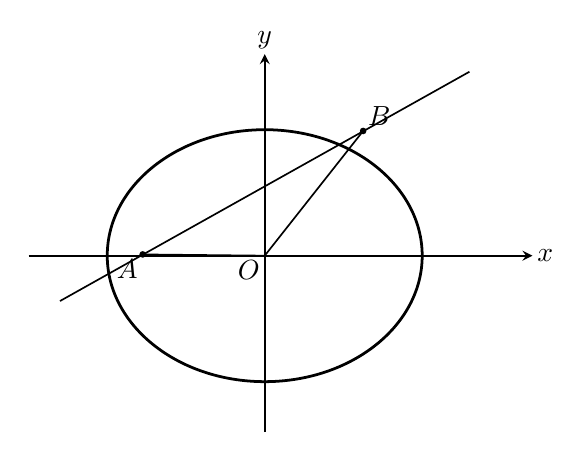
\begin{tikzpicture}[x=1.0cm, y=1.6cm, semithick,
  every node/.style={inner sep=1.5pt}]

  \draw[->,>=stealth] (-3.0,0) -- (3.4,0) node[right] {$x$};
  \draw[->,>=stealth] (0,-1.4) -- (0,1.6) node[above] {$y$};
  \node[below left] at (0,0) {$O$};

  % 椭圆 x^2/4+y^2=1
  \draw[line width=1pt] (0,0) ellipse (2 and 1);

  % 割线 y = 0.35x + 0.55（示意）
  \draw (-2.6,-0.36) -- (2.6,1.46);
  \coordinate (A) at (-1.55,0.01);
  \coordinate (B) at (1.25,0.99);
  \fill (A) circle (1.2pt);
  \fill (B) circle (1.2pt);
  \node[below left] at (A) {$A$};
  \node[above right] at (B) {$B$};

  \draw (A) -- (0,0) -- (B);
\end{tikzpicture}
\end{center}
\nopagebreak[4]
\Needspace{4\baselineskip}
\textbf{解析}

\Needspace{5\baselineskip}
（1）$k=0$ 时交点为 $\left(\pm2\sqrt{1-b^2},b\right)$，

\nopagebreak[4]
\[S=2b\sqrt{1-b^2}\leqslant1,\]

等号当 $b^2=\dfrac12$。

\Needspace{5\baselineskip}
（2）设交点横坐标 $x_1,x_2$，由联立得

\nopagebreak[4]
\[D=k^2+\frac14,\qquad |x_1-x_2|=\frac{\sqrt{4k^2+1-b^2}}{D}.\]

\Needspace{5\baselineskip}
于是

\nopagebreak[4]
\[|AB|=\sqrt{1+k^2}|x_1-x_2|=2,\qquad S=\frac12|b||x_1-x_2|=1.\]

\Needspace{5\baselineskip}
两式相除得 $b^2=1+k^2$，代回解得 $k^2=\dfrac12$，$b^2=\dfrac32$。故

\nopagebreak[4]
\[y=\pm\frac{\sqrt2}{2}x\pm\frac{\sqrt6}{2}.\]

\gkanswer{答案：（1）$1$；（2）$y=\pm\dfrac{\sqrt2}{2}x\pm\dfrac{\sqrt6}{2}$。}

\end{answer}
\begin{answer}
\gksolhead{21}{}

\textbf{题目}：

已知数列 $\{a_n\}$ 中的相邻两项 $a_{2k-1}$，$a_{2k}$ 是关于 $x$ 的方程 $x^2-(3k+2^k)x+3k\cdot2^k=0$ 的两个根，且 $a_{2k-1}\leqslant a_{2k}$（$k=1,2,3,\cdots$）。

（1）求 $a_1$，$a_3$，$a_5$，$a_7$；

（2）求数列 $\{a_n\}$ 的前 $2n$ 项和 $S_{2n}$；

（3）记 $f(n)=\dfrac12\left(\dfrac{|\sin n|}{\sin n}+3\right)$，$T_n=\dfrac{(-1)^{f(2)}}{a_1a_2}+\dfrac{(-1)^{f(3)}}{a_3a_4}+\dfrac{(-1)^{f(4)}}{a_5a_6}+\cdots+\dfrac{(-1)^{f(n+1)}}{a_{2n-1}a_{2n}}$，求证：$\dfrac16\leqslant T_n\leqslant\dfrac5{24}$（$n\in\mathbf N^*$）。

\Needspace{4\baselineskip}
\textbf{解析}

\Needspace{5\baselineskip}
（1）方程两根为 $3k$ 与 $2^k$，按大小排序：

\nopagebreak[4]
\[a_1=2,\ a_3=4,\ a_5=8,\ a_7=12.\]

\Needspace{5\baselineskip}
（2）每一对之和

\nopagebreak[4]
\[a_{2k-1}+a_{2k}=3k+2^k,\]

\Needspace{5\baselineskip}
故

\nopagebreak[4]
\[S_{2n}=\sum_{k=1}^n(3k+2^k)=\frac{3n(n+1)}2+2^{n+1}-2.\]

\Needspace{5\baselineskip}
（3）$n$ 为正整数时 $\sin n\neq0$，且

\nopagebreak[4]
\[f(n)=\begin{cases}2,&\sin n>0,\\1,&\sin n<0.\end{cases}\]

故 $(-1)^{f(k+1)}=1$ 当 $\sin(k+1)>0$，为 $-1$ 当 $\sin(k+1)<0$。

\Needspace{5\baselineskip}
由 $2<3<\pi$ 知 $\sin2>0$，$\sin3>0$。于是

\nopagebreak[4]
\[T_1=\frac1{a_1a_2}=\frac16,\qquad \frac{(-1)^{f(3)}}{a_3a_4}=\frac1{24}.\]

\Needspace{5\baselineskip}
记 $R_n=\displaystyle\sum_{k=3}^n\frac{(-1)^{f(k+1)}}{a_{2k-1}a_{2k}}$，则

\nopagebreak[4]
\[|R_n|\leqslant\sum_{k=3}^{\infty}\frac1{3k\cdot2^k}
<\frac1{72}+\frac1{192}+\frac1{480}+\cdots<\frac1{24}.\]

\Needspace{5\baselineskip}
因此

\nopagebreak[4]
\[T_n=\frac16+\frac1{24}+R_n,\]

\Needspace{5\baselineskip}
从而

\nopagebreak[4]
\[\frac16<T_n<\frac5{24},\]

故 $\dfrac16\leqslant T_n\leqslant\dfrac5{24}$。

\gkanswer{答案：（1）$a_1=2$，$a_3=4$，$a_5=8$，$a_7=12$；（2）$S_{2n}=\dfrac{3n(n+1)}2+2^{n+1}-2$；（3）证明见解析。}

\end{answer}
\begin{answer}
\gksolhead{22}{}

\textbf{题目}：

设 $f(x)=\dfrac{x^3}{3}$，对任意实数 $t$，记 $g_t(x)=t^2x-\dfrac23t^3$。

（1）求函数 $y=f(x)-g_8(x)$ 的单调区间；

（2）求证：

① 当 $x>0$ 时，$f(x)\geqslant g_t(x)$ 对任意实数 $t$ 成立；

② 有且仅有一个正实数 $x_0$，使得 $g_8(x_0)\geqslant g_t(x_0)$ 对任意实数 $t$ 成立。

\Needspace{4\baselineskip}
\textbf{解析}

\Needspace{5\baselineskip}
（1）$8^{2/3}=4$，故

\nopagebreak[4]
\[g_8(x)=4x-\frac{16}3,\]

\nopagebreak[4]
\[y=f(x)-g_8(x)=\frac{x^3}3-4x+\frac{16}3,\]

\nopagebreak[4]
\[y'=x^2-4.\]

故 $y$ 在 $(-\infty,-2)$ 与 $(2,+\infty)$ 上递增，在 $(-2,2)$ 上递减。

\Needspace{5\baselineskip}
（2）① 令 $u=t^{1/3}\geqslant0$，则

\nopagebreak[4]
\[g_t(x)=u^2x-\frac23u^3.\]

\Needspace{5\baselineskip}
要证

\nopagebreak[4]
\[\frac{x^3}3\geqslant u^2x-\frac23u^3,\]

\Needspace{5\baselineskip}
即

\nopagebreak[4]
\[h(u)=\frac23u^3-xu^2+\frac{x^3}3\geqslant0\quad(u\geqslant0).\]

\Needspace{5\baselineskip}
求导：

\nopagebreak[4]
\[h'(u)=2u^2-2xu=2u(u-x).\]

\Needspace{5\baselineskip}
$h$ 在 $(0,x)$ 上递减，在 $(x,+\infty)$ 上递增，而

\nopagebreak[4]
\[h(x)=\frac23x^3-x^3+\frac{x^3}3=0,\]

故 $u\geqslant0$ 时 $h(u)\geqslant h(x)=0$，不等式成立。

\Needspace{5\baselineskip}
② 由①，对固定的 $x>0$，$g_t(x)\leqslant f(x)$，且等号当 $u=x$，即 $t=x^3$ 时成立。因此

\nopagebreak[4]
\[g_8(x)\geqslant g_t(x)\ \text{\text{对一切} }t\ge0\]

\Needspace{5\baselineskip}
当且仅当 $g_8(x)=f(x)$，即 $8=x^3$，故唯一正解

\nopagebreak[4]
\[x_0=2.\]

（注：$8^{2/3}=4$，$g_8(x)=4x-\dfrac{16}3$；令 $g_8(x)=f(x)$ 得 $\dfrac{x^3}3-4x+\dfrac{16}3=0$，即 $(x-2)^2(x+4)=0$，唯一正根 $x_0=2$。）

\gkanswer{答案：（1）增区间 $(-\infty,-2)$，$(2,+\infty)$，减区间 $(-2,2)$；（2）证明见解析。}

\end{answer}